% Informe del laboratorio 2: planos v2.0 (ISA-5.1 / IEC 60617) y mockups de interfaces
% Compilar desde esta carpeta: pdflatex informe_lab02.tex (dos veces)
\documentclass[a4paper,11pt]{article}
% Preámbulo común de los informes de laboratorio (II/2026). Se incluye desde desarrollo/fuentes/laboratorios/labNN_*/
%   % Preámbulo común de los informes de laboratorio (II/2026). Se incluye desde desarrollo/fuentes/laboratorios/labNN_*/
%   % Preámbulo común de los informes de laboratorio (II/2026). Se incluye desde desarrollo/fuentes/laboratorios/labNN_*/
%   \input{../informe_comun}
\input{../../gemelo-digital/manual/estilo_manual}
\input{../../gemelo-digital/manual/tecnico/macros}
% Las rutas son relativas a la carpeta de cada informe (desarrollo/fuentes/laboratorios/labNN/): las fuentes
% (estilo, imágenes del manual, figuras y levantamiento) están en desarrollo/fuentes; los entregables públicos
% (planos, base de datos) cuatro niveles más arriba, en semestres/2026_II/.
\graphicspath{{../../../../documentacion/planos_isa/pid/}{../../../../documentacion/planos_isa/electrico/}{../../../../documentacion/manuales_inversa/}
  {../../../../database/mockups/}{../../../../database/documentacion/}{../../../../database/modelo/}{../../../../database/interfaz/}
  {../../gemelo-digital/manual/img/}{../../modelo-3d/informe/figuras/}{../../modelo-3d/levantamiento/}{../../../../../../global/fotos-planta/}}
\usepackage{pdflscape}
\lstset{showstringspaces=false}
% plano A3 en una página apaisada: \plano[página]{archivo}{leyenda}
\newcommand{\plano}[3][1]{\begin{landscape}\begin{figure}[p]\centering\includegraphics[page=#1, width=\linewidth, height=0.86\textwidth, keepaspectratio]{#2}\caption{#3}\end{figure}\end{landscape}}
\setlength{\headheight}{14pt}
\newcommand{\nlab}{}
\newcommand{\tlab}{}
% tipo de documento en la portada y el encabezado (los documentos de logros los redefinen)
\newcommand{\tipodoc}{Informe del Laboratorio Integrado}
\newcommand{\tipocab}{Informe del laboratorio}
\lhead{\small Brazo XK-JS1-1 · \tipocab{} \nlab}
\rhead{\small UMSA · II/2026}

% \portada{número}{título}{inicio}{entrega}{semanas}
\newcommand{\portada}[5]{%
\renewcommand{\nlab}{#1}%
\begin{titlepage}
\centering
\vspace*{0.6cm}
{\large Universidad Mayor de San Andrés · Facultad de Ingeniería\par}
{\large Carrera de Ingeniería Electrónica\par}
\vspace{0.8cm}
{\color{naranja!80!black}\rule{\linewidth}{1.5pt}\par}
\vspace{0.3cm}
{\Large \tipodoc{} Nº #1\par}
\vspace{0.2cm}
{\huge\bfseries #2\par}
\vspace{0.3cm}
{\color{naranja!80!black}\rule{\linewidth}{1.5pt}\par}
\vspace{0.8cm}
{\large Planta: brazo robótico XK-JS1-1 de 4 grados de libertad\par}
\vspace{0.3cm}
{\large ETN-902 Sistemas de Control II · ETN-1034 Aplicación de Técnicas de Control · ETN-1000 Bases de Datos\par}
\vspace{1cm}
\begin{tabular}{rl}
\textbf{Docente:} & Ing. Jorge Antonio Nava Amador\\
\textbf{Auxiliares:} & Limber Ajnota · Fabián Plata · Franz Choque\\
\textbf{Inicio de trabajo:} & #3\\
\textbf{Entrega:} & #4 (#5)\\
\end{tabular}
\vspace{1cm}

\begin{tabular}{ll}
\multicolumn{2}{l}{\textbf{Escuadra del brazo de 4 GDL}}\\[2pt]
Control (ETN-902 / ETN-1034): & Gabriel Andres Gomez Calla\\
 & Jose Lenin Mamani Choque\\
 & Miguel Alejandro Lima Huarachi\\
 & Román Abner Machicado Arequipa\\[2pt]
Cómputo (ETN-1000): & Miguel Alejandro Lima Huarachi\\
 & Marco Eduardo Chura Rondo\\
\end{tabular}
\vfill
{\small Repositorio: \url{https://github.com/GabAndGom/Brazo-de-4-grados-de-libertad}\par}
{\small La Paz, Bolivia · gestión II/2026\par}
\end{titlepage}
}

% Tabla de entregables (Definition of Done): \begin{dod} ... \end{dod}, filas: entregable & estado & evidencia\\
\newenvironment{dod}{\begin{center}\small\begin{longtable}{>{\raggedright}p{5.2cm} >{\raggedright}p{1.8cm} >{\raggedright\arraybackslash}p{7.6cm}}
\toprule \textbf{Entregable} & \textbf{Estado} & \textbf{Evidencia / observación}\\ \midrule \endhead}
{\bottomrule\end{longtable}\end{center}}

% Estilo común de los manuales del gemelo digital (se incluye con \input)
\usepackage{geometry}
\geometry{letterpaper, margin=2.2cm}
\usepackage[spanish, es-nodecimaldot, mexico]{babel}
\usepackage[utf8]{inputenc}
\usepackage[T1]{fontenc}
\usepackage{lmodern}
\usepackage{amsmath,amssymb}
\usepackage[table]{xcolor}
\definecolor{naranja}{RGB}{194,98,12}
\definecolor{rojo}{RGB}{192,57,43}
\definecolor{verde}{RGB}{30,120,70}
\definecolor{azulw}{RGB}{0,103,184}
\definecolor{azulg}{RGB}{70,90,120}
\definecolor{gris}{RGB}{242,242,242}
\definecolor{grisos}{RGB}{90,90,90}
\usepackage{booktabs,longtable,array,tabularx}
\usepackage{graphicx}
\usepackage{float}
\usepackage{caption}
\captionsetup{font=small, labelfont=bf}
\usepackage{tikz}
\usetikzlibrary{positioning,arrows.meta,fit,calc,shapes.geometric,decorations.pathreplacing,backgrounds}
\usepackage{enumitem}
\setlist{itemsep=2pt}
\usepackage{listings}
\lstset{basicstyle=\ttfamily\small, frame=single, backgroundcolor=\color{gris}, breaklines=true,
  columns=fullflexible, keepspaces=true, extendedchars=true, upquote=true,
  literate={á}{{\'a}}1 {é}{{\'e}}1 {í}{{\'i}}1 {ó}{{\'o}}1 {ú}{{\'u}}1 {ñ}{{\~n}}1 {Á}{{\'A}}1 {É}{{\'E}}1
           {Í}{{\'I}}1 {Ó}{{\'O}}1 {Ú}{{\'U}}1 {Ñ}{{\~N}}1 {ü}{{\"u}}1 {¿}{{?`}}1 {¡}{{!`}}1 {…}{{...}}3
           {θ}{{$\theta$}}1 {·}{{$\cdot$}}1 {«}{{\guillemotleft}}1 {»}{{\guillemotright}}1 {°}{{$^\circ$}}1}
\usepackage{hyperref}
\hypersetup{colorlinks=true, linkcolor=naranja, urlcolor=naranja}
\usepackage{fancyhdr}
\pagestyle{fancy}
\fancyhf{}
\cfoot{\small \thepage}
\newcommand{\codigo}[1]{\texttt{#1}}
\newcommand{\archivo}[1]{\textbf{\texttt{#1}}}
\newcommand{\aviso}[1]{\par\smallskip\noindent\colorbox{rojo!10}{\parbox{\dimexpr\linewidth-2\fboxsep}{\textbf{\color{rojo}Atención.} #1}}\par\smallskip}
\newcommand{\nota}[1]{\par\smallskip\noindent\colorbox{gris}{\parbox{\dimexpr\linewidth-2\fboxsep}{#1}}\par\smallskip}
\tikzset{
  marca/.style={circle, fill=naranja, text=white, font=\bfseries\footnotesize, inner sep=1.4pt, minimum size=4.6mm, draw=white, line width=0.8pt},
  caja/.style={draw, rounded corners=2pt, fill=gris, align=center, font=\small, minimum height=10mm, inner sep=4pt},
  cajab/.style={caja, fill=white},
  cajan/.style={caja, fill=naranja!14, draw=naranja!70!black},
  paso/.style={draw, rounded corners=2pt, fill=white, align=left, font=\small, text width=3.4cm, minimum height=15mm, inner sep=5pt},
  num/.style={circle, fill=naranja, text=white, font=\bfseries\small, inner sep=1.5pt, minimum size=6mm},
  flecha/.style={-{Stealth[length=2.2mm]}, thick},
  dflecha/.style={{Stealth[length=2.2mm]}-{Stealth[length=2.2mm]}, thick},
  etiq/.style={font=\scriptsize, align=center},
}
\DeclareRobustCommand{\num}[1]{\tikz[baseline=-0.7ex]\node[marca]{#1};}
% \captura{ancho}{archivo}{marcas en coordenadas 0-1 desde la esquina inferior izquierda}
\newcommand{\captura}[3]{%
  \begin{tikzpicture}
  \node[anchor=south west, inner sep=0, draw=black!25] (img) {\includegraphics[width=#1]{#2}};
  \begin{scope}[x={(img.south east)}, y={(img.north west)}]
  #3
  \end{scope}
  \end{tikzpicture}}
% ventana dibujada (consolas y diálogos): \ventana{ancho}{alto}{título}{contenido}
\newcommand{\ventana}[4]{%
\begin{tikzpicture}
\node[draw=black!50, fill=white, minimum width=#1, minimum height=#2, anchor=north west, inner sep=0] (v) at (0,0) {};
\fill[black!8] (v.north west) rectangle ($(v.north east)+(0,-6mm)$);
\node[anchor=west, font=\scriptsize] at ($(v.north west)+(2mm,-3mm)$) {#3};
\node[anchor=east, font=\scriptsize] at ($(v.north east)+(-2mm,-3mm)$) {--\quad$\square$\quad$\times$};
\node[anchor=north west, inner sep=3mm, text width=#1-6mm, font=\scriptsize\ttfamily, align=left] at ($(v.north west)+(0,-6mm)$) {#4};
\end{tikzpicture}}

% Macros del manual técnico: ladder, estados, código y rutas de imágenes
\usetikzlibrary{shapes.multipart}
\graphicspath{{../img/}{../../../../../../../global/fotos-planta/}{../../../modelo-3d/informe/figuras/}{../../../modelo-3d/levantamiento/}{../../../../../database/modelo/}{../../../../../documentacion/manuales_inversa/}{../../../../../documentacion/planos_isa/electrico/}{../../../../../database/interfaz/}}

\lstdefinestyle{py}{language=Python, keywordstyle=\color{azulg}\bfseries, commentstyle=\color{grisos}\itshape,
  stringstyle=\color{verde}, basicstyle=\ttfamily\scriptsize, numbers=left, numberstyle=\tiny\color{grisos}}
\lstdefinestyle{js}{language=Java, morekeywords={const,let,function,async,await,return,for,of,if,else}, keywordstyle=\color{azulg}\bfseries,
  commentstyle=\color{grisos}\itshape, stringstyle=\color{verde}, basicstyle=\ttfamily\scriptsize, numbers=left, numberstyle=\tiny\color{grisos}}
\lstdefinestyle{awl}{basicstyle=\ttfamily\tiny, commentstyle=\color{grisos}\itshape, morecomment=[l]{//},
  keywordstyle=\color{azulg}\bfseries, morekeywords={LD,LDN,A,AN,O,ON,EU,ED,S,R,MOVB,MOVW,MOVD,PLS,TON,CALL,CRET,LPS,LRD,LPP,ALD,OLD,FILL,LDW,LDB,LDD,AW,AD,AB,OW,OD},
  numbers=left, numberstyle=\tiny\color{grisos}, frame=single, backgroundcolor=\color{gris}}
\lstdefinestyle{sql}{language=SQL, keywordstyle=\color{azulg}\bfseries, commentstyle=\color{grisos}\itshape,
  stringstyle=\color{verde}, basicstyle=\ttfamily\tiny, numbers=left, numberstyle=\tiny\color{grisos},
  morekeywords={REFERENCES,SERIAL,SMALLSERIAL,BIGSERIAL,TIMESTAMPTZ,BOOLEAN,INET,RETURNS,TRIGGER,LANGUAGE,DECLARE,RAISE,EXCEPTION,VIEW,INDEX}}

\tikzset{
  ld/.style={line width=0.7pt},
  pics/na/.style={code={\fill[white](-0.12,-0.26) rectangle (0.12,0.26);
     \draw[thick](-0.1,-0.24)--(-0.1,0.24)(0.1,-0.24)--(0.1,0.24);
     \node[font=\scriptsize\ttfamily, above] at (0,0.22){#1};}},
  pics/nc/.style={code={\fill[white](-0.12,-0.26) rectangle (0.12,0.26);
     \draw[thick](-0.1,-0.24)--(-0.1,0.24)(0.1,-0.24)--(0.1,0.24);\draw(-0.17,-0.24)--(0.17,0.24);
     \node[font=\scriptsize\ttfamily, above] at (0,0.22){#1};}},
  pics/pf/.style={code={\fill[white](-0.12,-0.26) rectangle (0.12,0.26);
     \draw[thick](-0.1,-0.24)--(-0.1,0.24)(0.1,-0.24)--(0.1,0.24);
     \node[font=\tiny\bfseries] at (0,0){P};}},
  pics/cmp/.style n args={3}{code={\fill[white](-0.12,-0.26) rectangle (0.12,0.26);
     \draw[thick](-0.1,-0.24)--(-0.1,0.24)(0.1,-0.24)--(0.1,0.24);
     \node[font=\tiny\ttfamily] at (0,0){#2};
     \node[font=\scriptsize\ttfamily, above] at (0,0.22){#1};
     \node[font=\scriptsize\ttfamily, below] at (0,-0.22){#3};}},
  pics/bob/.style n args={3}{code={\fill[white](-0.2,-0.26) rectangle (0.2,0.26);
     \draw[thick](-0.05,0.24) arc (110:250:0.255);\draw[thick](0.05,0.24) arc (70:-70:0.255);
     \node[font=\tiny\bfseries] at (0,0){#2};
     \node[font=\scriptsize\ttfamily, above] at (0,0.22){#1};
     \node[font=\scriptsize\ttfamily, below] at (0,-0.22){#3};}},
  fb/.style={draw, fill=white, font=\scriptsize\ttfamily, align=left, inner sep=3pt, anchor=west},
  barra/.style={line width=2pt},
  estado/.style={draw, rounded corners=3pt, fill=white, align=center, font=\scriptsize, minimum width=22mm, minimum height=10mm, inner sep=3pt},
  estadon/.style={estado, fill=naranja!14, draw=naranja!70!black},
  trans/.style={font=\scriptsize, align=center, fill=white, inner sep=1pt},
  lugar/.style={circle, draw, thick, minimum size=7mm, fill=white},
  transicion/.style={rectangle, fill=black, minimum width=1.6mm, minimum height=7mm, inner sep=0},
  tabla/.style={rectangle split, rectangle split parts=2, draw, fill=white, font=\tiny\ttfamily, align=left, inner sep=2pt, rounded corners=1pt, text width=33mm},
}
\newcommand{\pendiente}[1]{\par\smallskip\noindent\colorbox{naranja!12}{\parbox{\dimexpr\linewidth-2\fboxsep}{\textbf{\color{naranja!80!black}Pendiente.} #1}}\par\smallskip}
\newcommand{\cumple}{\textcolor{verde}{\textbf{cumplido}}}
\newcommand{\parcial}{\textcolor{naranja}{\textbf{parcial}}}
\newcommand{\falta}{\textcolor{rojo}{\textbf{pendiente}}}

% Las rutas son relativas a la carpeta de cada informe (desarrollo/fuentes/laboratorios/labNN/): las fuentes
% (estilo, imágenes del manual, figuras y levantamiento) están en desarrollo/fuentes; los entregables públicos
% (planos, base de datos) cuatro niveles más arriba, en semestres/2026_II/.
\graphicspath{{../../../../documentacion/planos_isa/pid/}{../../../../documentacion/planos_isa/electrico/}{../../../../documentacion/manuales_inversa/}
  {../../../../database/mockups/}{../../../../database/documentacion/}{../../../../database/modelo/}{../../../../database/interfaz/}
  {../../gemelo-digital/manual/img/}{../../modelo-3d/informe/figuras/}{../../modelo-3d/levantamiento/}{../../../../../../global/fotos-planta/}}
\usepackage{pdflscape}
\lstset{showstringspaces=false}
% plano A3 en una página apaisada: \plano[página]{archivo}{leyenda}
\newcommand{\plano}[3][1]{\begin{landscape}\begin{figure}[p]\centering\includegraphics[page=#1, width=\linewidth, height=0.86\textwidth, keepaspectratio]{#2}\caption{#3}\end{figure}\end{landscape}}
\setlength{\headheight}{14pt}
\newcommand{\nlab}{}
\newcommand{\tlab}{}
% tipo de documento en la portada y el encabezado (los documentos de logros los redefinen)
\newcommand{\tipodoc}{Informe del Laboratorio Integrado}
\newcommand{\tipocab}{Informe del laboratorio}
\lhead{\small Brazo XK-JS1-1 · \tipocab{} \nlab}
\rhead{\small UMSA · II/2026}

% \portada{número}{título}{inicio}{entrega}{semanas}
\newcommand{\portada}[5]{%
\renewcommand{\nlab}{#1}%
\begin{titlepage}
\centering
\vspace*{0.6cm}
{\large Universidad Mayor de San Andrés · Facultad de Ingeniería\par}
{\large Carrera de Ingeniería Electrónica\par}
\vspace{0.8cm}
{\color{naranja!80!black}\rule{\linewidth}{1.5pt}\par}
\vspace{0.3cm}
{\Large \tipodoc{} Nº #1\par}
\vspace{0.2cm}
{\huge\bfseries #2\par}
\vspace{0.3cm}
{\color{naranja!80!black}\rule{\linewidth}{1.5pt}\par}
\vspace{0.8cm}
{\large Planta: brazo robótico XK-JS1-1 de 4 grados de libertad\par}
\vspace{0.3cm}
{\large ETN-902 Sistemas de Control II · ETN-1034 Aplicación de Técnicas de Control · ETN-1000 Bases de Datos\par}
\vspace{1cm}
\begin{tabular}{rl}
\textbf{Docente:} & Ing. Jorge Antonio Nava Amador\\
\textbf{Auxiliares:} & Limber Ajnota · Fabián Plata · Franz Choque\\
\textbf{Inicio de trabajo:} & #3\\
\textbf{Entrega:} & #4 (#5)\\
\end{tabular}
\vspace{1cm}

\begin{tabular}{ll}
\multicolumn{2}{l}{\textbf{Escuadra del brazo de 4 GDL}}\\[2pt]
Control (ETN-902 / ETN-1034): & Gabriel Andres Gomez Calla\\
 & Jose Lenin Mamani Choque\\
 & Miguel Alejandro Lima Huarachi\\
 & Román Abner Machicado Arequipa\\[2pt]
Cómputo (ETN-1000): & Miguel Alejandro Lima Huarachi\\
 & Marco Eduardo Chura Rondo\\
\end{tabular}
\vfill
{\small Repositorio: \url{https://github.com/GabAndGom/Brazo-de-4-grados-de-libertad}\par}
{\small La Paz, Bolivia · gestión II/2026\par}
\end{titlepage}
}

% Tabla de entregables (Definition of Done): \begin{dod} ... \end{dod}, filas: entregable & estado & evidencia\\
\newenvironment{dod}{\begin{center}\small\begin{longtable}{>{\raggedright}p{5.2cm} >{\raggedright}p{1.8cm} >{\raggedright\arraybackslash}p{7.6cm}}
\toprule \textbf{Entregable} & \textbf{Estado} & \textbf{Evidencia / observación}\\ \midrule \endhead}
{\bottomrule\end{longtable}\end{center}}

% Estilo común de los manuales del gemelo digital (se incluye con \input)
\usepackage{geometry}
\geometry{letterpaper, margin=2.2cm}
\usepackage[spanish, es-nodecimaldot, mexico]{babel}
\usepackage[utf8]{inputenc}
\usepackage[T1]{fontenc}
\usepackage{lmodern}
\usepackage{amsmath,amssymb}
\usepackage[table]{xcolor}
\definecolor{naranja}{RGB}{194,98,12}
\definecolor{rojo}{RGB}{192,57,43}
\definecolor{verde}{RGB}{30,120,70}
\definecolor{azulw}{RGB}{0,103,184}
\definecolor{azulg}{RGB}{70,90,120}
\definecolor{gris}{RGB}{242,242,242}
\definecolor{grisos}{RGB}{90,90,90}
\usepackage{booktabs,longtable,array,tabularx}
\usepackage{graphicx}
\usepackage{float}
\usepackage{caption}
\captionsetup{font=small, labelfont=bf}
\usepackage{tikz}
\usetikzlibrary{positioning,arrows.meta,fit,calc,shapes.geometric,decorations.pathreplacing,backgrounds}
\usepackage{enumitem}
\setlist{itemsep=2pt}
\usepackage{listings}
\lstset{basicstyle=\ttfamily\small, frame=single, backgroundcolor=\color{gris}, breaklines=true,
  columns=fullflexible, keepspaces=true, extendedchars=true, upquote=true,
  literate={á}{{\'a}}1 {é}{{\'e}}1 {í}{{\'i}}1 {ó}{{\'o}}1 {ú}{{\'u}}1 {ñ}{{\~n}}1 {Á}{{\'A}}1 {É}{{\'E}}1
           {Í}{{\'I}}1 {Ó}{{\'O}}1 {Ú}{{\'U}}1 {Ñ}{{\~N}}1 {ü}{{\"u}}1 {¿}{{?`}}1 {¡}{{!`}}1 {…}{{...}}3
           {θ}{{$\theta$}}1 {·}{{$\cdot$}}1 {«}{{\guillemotleft}}1 {»}{{\guillemotright}}1 {°}{{$^\circ$}}1}
\usepackage{hyperref}
\hypersetup{colorlinks=true, linkcolor=naranja, urlcolor=naranja}
\usepackage{fancyhdr}
\pagestyle{fancy}
\fancyhf{}
\cfoot{\small \thepage}
\newcommand{\codigo}[1]{\texttt{#1}}
\newcommand{\archivo}[1]{\textbf{\texttt{#1}}}
\newcommand{\aviso}[1]{\par\smallskip\noindent\colorbox{rojo!10}{\parbox{\dimexpr\linewidth-2\fboxsep}{\textbf{\color{rojo}Atención.} #1}}\par\smallskip}
\newcommand{\nota}[1]{\par\smallskip\noindent\colorbox{gris}{\parbox{\dimexpr\linewidth-2\fboxsep}{#1}}\par\smallskip}
\tikzset{
  marca/.style={circle, fill=naranja, text=white, font=\bfseries\footnotesize, inner sep=1.4pt, minimum size=4.6mm, draw=white, line width=0.8pt},
  caja/.style={draw, rounded corners=2pt, fill=gris, align=center, font=\small, minimum height=10mm, inner sep=4pt},
  cajab/.style={caja, fill=white},
  cajan/.style={caja, fill=naranja!14, draw=naranja!70!black},
  paso/.style={draw, rounded corners=2pt, fill=white, align=left, font=\small, text width=3.4cm, minimum height=15mm, inner sep=5pt},
  num/.style={circle, fill=naranja, text=white, font=\bfseries\small, inner sep=1.5pt, minimum size=6mm},
  flecha/.style={-{Stealth[length=2.2mm]}, thick},
  dflecha/.style={{Stealth[length=2.2mm]}-{Stealth[length=2.2mm]}, thick},
  etiq/.style={font=\scriptsize, align=center},
}
\DeclareRobustCommand{\num}[1]{\tikz[baseline=-0.7ex]\node[marca]{#1};}
% \captura{ancho}{archivo}{marcas en coordenadas 0-1 desde la esquina inferior izquierda}
\newcommand{\captura}[3]{%
  \begin{tikzpicture}
  \node[anchor=south west, inner sep=0, draw=black!25] (img) {\includegraphics[width=#1]{#2}};
  \begin{scope}[x={(img.south east)}, y={(img.north west)}]
  #3
  \end{scope}
  \end{tikzpicture}}
% ventana dibujada (consolas y diálogos): \ventana{ancho}{alto}{título}{contenido}
\newcommand{\ventana}[4]{%
\begin{tikzpicture}
\node[draw=black!50, fill=white, minimum width=#1, minimum height=#2, anchor=north west, inner sep=0] (v) at (0,0) {};
\fill[black!8] (v.north west) rectangle ($(v.north east)+(0,-6mm)$);
\node[anchor=west, font=\scriptsize] at ($(v.north west)+(2mm,-3mm)$) {#3};
\node[anchor=east, font=\scriptsize] at ($(v.north east)+(-2mm,-3mm)$) {--\quad$\square$\quad$\times$};
\node[anchor=north west, inner sep=3mm, text width=#1-6mm, font=\scriptsize\ttfamily, align=left] at ($(v.north west)+(0,-6mm)$) {#4};
\end{tikzpicture}}

% Macros del manual técnico: ladder, estados, código y rutas de imágenes
\usetikzlibrary{shapes.multipart}
\graphicspath{{../img/}{../../../../../../../global/fotos-planta/}{../../../modelo-3d/informe/figuras/}{../../../modelo-3d/levantamiento/}{../../../../../database/modelo/}{../../../../../documentacion/manuales_inversa/}{../../../../../documentacion/planos_isa/electrico/}{../../../../../database/interfaz/}}

\lstdefinestyle{py}{language=Python, keywordstyle=\color{azulg}\bfseries, commentstyle=\color{grisos}\itshape,
  stringstyle=\color{verde}, basicstyle=\ttfamily\scriptsize, numbers=left, numberstyle=\tiny\color{grisos}}
\lstdefinestyle{js}{language=Java, morekeywords={const,let,function,async,await,return,for,of,if,else}, keywordstyle=\color{azulg}\bfseries,
  commentstyle=\color{grisos}\itshape, stringstyle=\color{verde}, basicstyle=\ttfamily\scriptsize, numbers=left, numberstyle=\tiny\color{grisos}}
\lstdefinestyle{awl}{basicstyle=\ttfamily\tiny, commentstyle=\color{grisos}\itshape, morecomment=[l]{//},
  keywordstyle=\color{azulg}\bfseries, morekeywords={LD,LDN,A,AN,O,ON,EU,ED,S,R,MOVB,MOVW,MOVD,PLS,TON,CALL,CRET,LPS,LRD,LPP,ALD,OLD,FILL,LDW,LDB,LDD,AW,AD,AB,OW,OD},
  numbers=left, numberstyle=\tiny\color{grisos}, frame=single, backgroundcolor=\color{gris}}
\lstdefinestyle{sql}{language=SQL, keywordstyle=\color{azulg}\bfseries, commentstyle=\color{grisos}\itshape,
  stringstyle=\color{verde}, basicstyle=\ttfamily\tiny, numbers=left, numberstyle=\tiny\color{grisos},
  morekeywords={REFERENCES,SERIAL,SMALLSERIAL,BIGSERIAL,TIMESTAMPTZ,BOOLEAN,INET,RETURNS,TRIGGER,LANGUAGE,DECLARE,RAISE,EXCEPTION,VIEW,INDEX}}

\tikzset{
  ld/.style={line width=0.7pt},
  pics/na/.style={code={\fill[white](-0.12,-0.26) rectangle (0.12,0.26);
     \draw[thick](-0.1,-0.24)--(-0.1,0.24)(0.1,-0.24)--(0.1,0.24);
     \node[font=\scriptsize\ttfamily, above] at (0,0.22){#1};}},
  pics/nc/.style={code={\fill[white](-0.12,-0.26) rectangle (0.12,0.26);
     \draw[thick](-0.1,-0.24)--(-0.1,0.24)(0.1,-0.24)--(0.1,0.24);\draw(-0.17,-0.24)--(0.17,0.24);
     \node[font=\scriptsize\ttfamily, above] at (0,0.22){#1};}},
  pics/pf/.style={code={\fill[white](-0.12,-0.26) rectangle (0.12,0.26);
     \draw[thick](-0.1,-0.24)--(-0.1,0.24)(0.1,-0.24)--(0.1,0.24);
     \node[font=\tiny\bfseries] at (0,0){P};}},
  pics/cmp/.style n args={3}{code={\fill[white](-0.12,-0.26) rectangle (0.12,0.26);
     \draw[thick](-0.1,-0.24)--(-0.1,0.24)(0.1,-0.24)--(0.1,0.24);
     \node[font=\tiny\ttfamily] at (0,0){#2};
     \node[font=\scriptsize\ttfamily, above] at (0,0.22){#1};
     \node[font=\scriptsize\ttfamily, below] at (0,-0.22){#3};}},
  pics/bob/.style n args={3}{code={\fill[white](-0.2,-0.26) rectangle (0.2,0.26);
     \draw[thick](-0.05,0.24) arc (110:250:0.255);\draw[thick](0.05,0.24) arc (70:-70:0.255);
     \node[font=\tiny\bfseries] at (0,0){#2};
     \node[font=\scriptsize\ttfamily, above] at (0,0.22){#1};
     \node[font=\scriptsize\ttfamily, below] at (0,-0.22){#3};}},
  fb/.style={draw, fill=white, font=\scriptsize\ttfamily, align=left, inner sep=3pt, anchor=west},
  barra/.style={line width=2pt},
  estado/.style={draw, rounded corners=3pt, fill=white, align=center, font=\scriptsize, minimum width=22mm, minimum height=10mm, inner sep=3pt},
  estadon/.style={estado, fill=naranja!14, draw=naranja!70!black},
  trans/.style={font=\scriptsize, align=center, fill=white, inner sep=1pt},
  lugar/.style={circle, draw, thick, minimum size=7mm, fill=white},
  transicion/.style={rectangle, fill=black, minimum width=1.6mm, minimum height=7mm, inner sep=0},
  tabla/.style={rectangle split, rectangle split parts=2, draw, fill=white, font=\tiny\ttfamily, align=left, inner sep=2pt, rounded corners=1pt, text width=33mm},
}
\newcommand{\pendiente}[1]{\par\smallskip\noindent\colorbox{naranja!12}{\parbox{\dimexpr\linewidth-2\fboxsep}{\textbf{\color{naranja!80!black}Pendiente.} #1}}\par\smallskip}
\newcommand{\cumple}{\textcolor{verde}{\textbf{cumplido}}}
\newcommand{\parcial}{\textcolor{naranja}{\textbf{parcial}}}
\newcommand{\falta}{\textcolor{rojo}{\textbf{pendiente}}}

% Las rutas son relativas a la carpeta de cada informe (desarrollo/fuentes/laboratorios/labNN/): las fuentes
% (estilo, imágenes del manual, figuras y levantamiento) están en desarrollo/fuentes; los entregables públicos
% (planos, base de datos) cuatro niveles más arriba, en semestres/2026_II/.
\graphicspath{{../../../../documentacion/planos_isa/pid/}{../../../../documentacion/planos_isa/electrico/}{../../../../documentacion/manuales_inversa/}
  {../../../../database/mockups/}{../../../../database/documentacion/}{../../../../database/modelo/}{../../../../database/interfaz/}
  {../../gemelo-digital/manual/img/}{../../modelo-3d/informe/figuras/}{../../modelo-3d/levantamiento/}{../../../../../../global/fotos-planta/}}
\usepackage{pdflscape}
\lstset{showstringspaces=false}
% plano A3 en una página apaisada: \plano[página]{archivo}{leyenda}
\newcommand{\plano}[3][1]{\begin{landscape}\begin{figure}[p]\centering\includegraphics[page=#1, width=\linewidth, height=0.86\textwidth, keepaspectratio]{#2}\caption{#3}\end{figure}\end{landscape}}
\setlength{\headheight}{14pt}
\newcommand{\nlab}{}
\newcommand{\tlab}{}
% tipo de documento en la portada y el encabezado (los documentos de logros los redefinen)
\newcommand{\tipodoc}{Informe del Laboratorio Integrado}
\newcommand{\tipocab}{Informe del laboratorio}
\lhead{\small Brazo XK-JS1-1 · \tipocab{} \nlab}
\rhead{\small UMSA · II/2026}

% \portada{número}{título}{inicio}{entrega}{semanas}
\newcommand{\portada}[5]{%
\renewcommand{\nlab}{#1}%
\begin{titlepage}
\centering
\vspace*{0.6cm}
{\large Universidad Mayor de San Andrés · Facultad de Ingeniería\par}
{\large Carrera de Ingeniería Electrónica\par}
\vspace{0.8cm}
{\color{naranja!80!black}\rule{\linewidth}{1.5pt}\par}
\vspace{0.3cm}
{\Large \tipodoc{} Nº #1\par}
\vspace{0.2cm}
{\huge\bfseries #2\par}
\vspace{0.3cm}
{\color{naranja!80!black}\rule{\linewidth}{1.5pt}\par}
\vspace{0.8cm}
{\large Planta: brazo robótico XK-JS1-1 de 4 grados de libertad\par}
\vspace{0.3cm}
{\large ETN-902 Sistemas de Control II · ETN-1034 Aplicación de Técnicas de Control · ETN-1000 Bases de Datos\par}
\vspace{1cm}
\begin{tabular}{rl}
\textbf{Docente:} & Ing. Jorge Antonio Nava Amador\\
\textbf{Auxiliares:} & Limber Ajnota · Fabián Plata · Franz Choque\\
\textbf{Inicio de trabajo:} & #3\\
\textbf{Entrega:} & #4 (#5)\\
\end{tabular}
\vspace{1cm}

\begin{tabular}{ll}
\multicolumn{2}{l}{\textbf{Escuadra del brazo de 4 GDL}}\\[2pt]
Control (ETN-902 / ETN-1034): & Gabriel Andres Gomez Calla\\
 & Jose Lenin Mamani Choque\\
 & Miguel Alejandro Lima Huarachi\\
 & Román Abner Machicado Arequipa\\[2pt]
Cómputo (ETN-1000): & Miguel Alejandro Lima Huarachi\\
 & Marco Eduardo Chura Rondo\\
\end{tabular}
\vfill
{\small Repositorio: \url{https://github.com/GabAndGom/Brazo-de-4-grados-de-libertad}\par}
{\small La Paz, Bolivia · gestión II/2026\par}
\end{titlepage}
}

% Tabla de entregables (Definition of Done): \begin{dod} ... \end{dod}, filas: entregable & estado & evidencia\\
\newenvironment{dod}{\begin{center}\small\begin{longtable}{>{\raggedright}p{5.2cm} >{\raggedright}p{1.8cm} >{\raggedright\arraybackslash}p{7.6cm}}
\toprule \textbf{Entregable} & \textbf{Estado} & \textbf{Evidencia / observación}\\ \midrule \endhead}
{\bottomrule\end{longtable}\end{center}}


\begin{document}
\portada{2}{Planos de ingeniería versión 2.0 y diseño de interfaces}{martes 18 de agosto de 2026}{martes 1 de septiembre de 2026}{semanas 3 y 4}

\tableofcontents
\newpage

\section{Objetivos}
\subsection{Mención Control Automático (ETN-902 / ETN-1034)}
\begin{itemize}
\item \textbf{Normalización internacional}: aplicar ANSI/ISA-S5.1-2009 en el P\&ID e IEC 60617 en los esquemas eléctricos de potencia y mando.
\item \textbf{Documentación de ingeniería}: planos con capas, símbolos normalizados y referencias cruzadas.
\item \textbf{Estratificación de versiones (Kaizen)}: tomar los planos auditados en el laboratorio 1 y generar la versión 2.0, corrigiendo las discrepancias físicas.
\end{itemize}
\subsection{Mención Sistemas Computacionales (ETN-1000)}
\begin{itemize}
\item \textbf{Modelado de interfaces}: wireframes y mockups de la HMI de planta y del dashboard web.
\item \textbf{Flujos de captura}: jerarquía de navegación y cuadro de los elementos visuales que se guardarán en el backend.
\end{itemize}

\section{Alcance y justificación SDLC}
El trabajo se hizo en gabinete, sin modificar el hardware. Cada plano y cada pantalla es la etapa de \emph{diseño} del ciclo de vida: toma como requerimiento lo que se encontró en la auditoría del laboratorio 1 y alimenta el modelo de datos del laboratorio 3.

\begin{figure}[H]
\centering
\begin{tikzpicture}[node distance=4mm and 7mm, every node/.style={font=\scriptsize}]
\node[paso] (a) {\textbf{Lab 1}\\auditoría cable por cable\\reporte de discrepancias};
\node[paso, right=of a] (b) {\textbf{Lab 2 (este)}\\P\&ID y eléctrico v2.0\\mockups y cuadro de campos};
\node[paso, right=of b] (c) {\textbf{Lab 3}\\modelo E-R con los mismos tags ISA};
\node[paso, right=of c] (d) {\textbf{Fases 2 y 3}\\base de datos, middleware, dashboard};
\draw[flecha] (a) -- (b); \draw[flecha] (b) -- (c); \draw[flecha] (c) -- (d);
\end{tikzpicture}
\caption{Lugar del laboratorio 2 en el ciclo de vida del proyecto.}
\end{figure}

\section{ETN-902: diagrama P\&ID versión 2.0}
\subsection{Levantamiento según ISA-5.1}
El P\&ID (plano P\&ID-B4G-01) representa el brazo como proceso mecánico: cuatro grados de libertad (base, carro X, carro Y y garra) movidos por motores paso a paso, con supervisión discreta mediante finales de carrera y un sensor inductivo.

\plano{brazo_pid_v2.pdf}{P\&ID versión 2.0 (\codigo{documentacion/planos\_isa/pid/brazo\_pid\_v2.dwg}, también en DXF y PDF).}

\paragraph{Calibre de líneas.} Las señales eléctricas van en trazo discontinuo de 0,25~mm (capa \codigo{SENAL}) y los enlaces mecánicos o de proceso en trazo continuo de 1,0~mm (capa \codigo{PROCESO}), como pide la guía. El enlace PPI con la PC se dibuja como enlace de datos (línea con círculos).

\paragraph{Ubicación de cada instrumento.} Se usan los cuatro símbolos de la norma: círculo simple (instrumento en campo: finales de carrera, drivers), círculo con línea (instrumento en el panel accesible al operador: botonera y selector), rombo en cuadrado (función lógica compartida del PLC) y círculo en cuadrado (pantalla compartida: el gemelo digital en la PC).

\subsection{Identificación de lazos}
\begin{center}\small
\begin{tabularx}{\linewidth}{c >{\raggedright}p{2.6cm} >{\ttfamily\raggedright\arraybackslash}X}
\toprule
\textbf{Lazo} & \textbf{Grado de libertad} & \textrm{\textbf{Instrumentos (tags ISA-5.1)}}\\
\midrule
100 & general & HS-100 (selector man/auto, I0.5), HS-100P (paro, I0.6), ZY-100 (tren compartido, Q0.1), ZI-100 (gemelo digital)\\
101 & base $\theta$ & ZS-101 (inductivo, I0.0), HS-101A/B (jog, I1.0/I1.1), ZIC-101, ZY-101 (driver 2M530, Q0.0/Q0.2), M-101\\
102 & carro X & ZSL/ZSH-102 (finales, I0.1/I0.2), HS-102A/B (I1.2/I1.3), ZIC-102, ZY-102 (driver 2M542, Q0.3), K1 (Q0.5), M-102\\
103 & carro Y & ZSL/ZSH-103 (finales, I0.3/I0.4), HS-103A/B (I1.4/I1.5), ZIC-103, ZY-103 (driver 2M542, Q0.4), K2 (Q0.6), M-103\\
104 & garra & HS-104 (start/S1, I0.7), XC-104, XY-104 (relé K3, Q0.7), XV-104 (solenoide 24 V)\\
\bottomrule
\end{tabularx}
\end{center}
La letra \textbf{Z} (posición) es la variable medida de los lazos 101 a 103: el brazo controla posiciones. La garra es un actuador todo o nada, por eso usa la letra \textbf{X} (sin clasificar). El P\&ID deja explícito que no hay realimentación continua: la posición se estima contando pulsos y solo los finales y el inductivo dan información real de posición (lazo abierto con supervisión discreta).

\section{ETN-1034: esquema eléctrico industrial versión 2.0}
El esquema eléctrico (plano E-B4G-01) separa la potencia del mando en dos hojas, como exige la guía.

\plano[1]{brazo_electrico_v2.pdf}{Hoja 1, potencia: alimentación de 220~V, disyuntor -Q1, fuente -G1, fusibles, barras de 24~V y 5~V, drivers -A1 a -A3 y motores -M1 a -M3.}

\plano[2]{brazo_electrico_v2.pdf}{Hoja 2, mando: PLC -A4 con todos sus bornes de entrada y salida, relés -K1 a -K3, solenoide -Y1, sensores y botonera, y tabla de E/S con tags ISA.}

\subsection{Referencias cruzadas y rotulación}
\begin{itemize}
\item \textbf{Referencias cruzadas} con la convención \emph{hoja.columna}: por ejemplo, la bobina de -K1 (hoja 2, columna 4) indica que su contacto está en /2.1, y el PUL+ del driver -A2 indica que viene de Q0.1 a través de K1 (/2.1).
\item \textbf{Números de cable}: W0.0 a W0.4 para las salidas del PLC y E0.0 a E1.5 para las entradas.
\item \textbf{Bornes}: cada borne del PLC (1M, 1L+, Q0.0\dots Q1.1, 2M, I0.0\dots I1.5) y de los drivers (V+, GND, A$\pm$, B$\pm$, PUL$\pm$, DIR$\pm$, ENA$\pm$) está dibujado y rotulado.
\item \textbf{Capas}: 19 capas con color propio (potencia, 24~V, 0~V, 5~V, mando, bornes, números de cable, referencias, revisión, cajetín\dots).
\end{itemize}

\subsection{Correcciones Kaizen respecto del plano histórico}
\begin{center}\small
\begin{tabularx}{\linewidth}{c >{\raggedright\arraybackslash}X}
\toprule
\textbf{Nº} & \textbf{Corrección (verificada con el PLC en marcha)}\\
\midrule
1 & Finales de carrera en I0.1--I0.4 (X atrás/adelante, Y abajo/arriba); el inductivo de la base en I0.0.\\
2 & El tren de pulsos de X e Y sale de una sola salida (Q0.1) y lo reparten los relés K1 (Q0.5) y K2 (Q0.6).\\
3 & Las salidas de dirección Q0.3 (X) y Q0.4 (Y) están conectadas a DIR+; en el plano histórico figuraban sin conexión.\\
4 & El relé K3 se redibujó: bobina por Q0.7 y contacto hacia el solenoide de la garra.\\
5 & Start en paralelo con S1 (I0.7) y Stop en paralelo con S2 (I1.0).\\
6 & Drivers identificados: X e Y con 2M542 (DIP para 1000 pulsos/vuelta), base con 2M530; motores NEMA 23 (2,8~A) en X e Y y NEMA 17 (1,2~A) en la base.\\
7 & Lazos numerados 100 a 104 con tags ISA-5.1 y enlace PPI al gemelo digital.\\
\bottomrule
\end{tabularx}
\end{center}

\aviso{Quedan puntos marcados como SUPUESTO en el plano porque no se pudieron ver sin desarmar el tablero: el común de entradas 1M/2M (se dibujó a +24~V por ser NPN el sensor inductivo), el nivel de PUL/DIR (entradas optoacopladas de 5~V alimentadas con 24~V), la tabla DIP del 2M530 y la numeración del zócalo de los relés. Se deben verificar con multímetro antes de dar el plano por definitivo.}

\paragraph{Herramienta.} Los planos se generan con un script (\codigo{generar\_planos\_v2.py}) que escribe DXF con capas, tipos de línea y textos, y se convierten a DWG de AutoCAD 2018 con ODA File Converter. Así el plano se puede regenerar y versionar como código. Los símbolos se dibujaron según IEC 60617 e ISA-5.1, pero no son los bloques de la librería de AutoCAD Electrical que provee el auxiliar: si el docente lo exige, el DWG se puede abrir en AutoCAD Electrical y reemplazar los símbolos por los bloques de la librería.

\section{ETN-1000: mockups, organigrama y cuadro de campos}
\subsection{Adaptación del enunciado}
La planta no tiene una HMI física (PanelView). El equipo de cómputo adaptó la «pantalla HMI de planta» a una aplicación de escritorio en la PC conectada al PLC, manteniendo los dos entornos que pide la guía: la interfaz local de operación y el dashboard web analítico.

\begin{figure}[H]
\centering
\includegraphics[page=3, width=0.49\linewidth]{lab2_mockups_y_organigrama.pdf}\hfill
\includegraphics[page=4, width=0.49\linewidth]{lab2_mockups_y_organigrama.pdf}
\caption{Mockups del equipo de cómputo: interfaz local de planta (izquierda) y dashboard del ERP web (derecha).}
\end{figure}

\begin{figure}[H]
\centering
\includegraphics[page=5, width=0.62\linewidth]{lab2_mockups_y_organigrama.pdf}
\caption{Organigrama de vistas y navegación: autenticación, interfaz local y dashboard.}
\end{figure}

\subsection{Cuadro descriptivo de campos de almacenamiento}
\begin{center}\small
\begin{tabularx}{\linewidth}{>{\raggedright}p{3.6cm} >{\raggedright}p{2.2cm} >{\raggedright\arraybackslash}X}
\toprule
\textbf{Elemento visual} & \textbf{Tipo de dato} & \textbf{Columna en la base (laboratorio 3)}\\
\midrule
Selector manual / auto & bit & \codigo{estado\_io.valor} de HS-100 (I0.5)\\
Parada de emergencia & bit + evento & \codigo{orden.tipo = 'emergencia'} y \codigo{evento\_alarma} (paro)\\
Pinza (accionar) & bit & \codigo{orden.tipo = 'garra'}; estado en XY-104 (Q0.7)\\
Seis botones de movimiento & bits + destino & \codigo{orden} (\codigo{mover}) y \codigo{orden\_parametro} (destino por eje)\\
Sensores 1--4 e inductivo & bit & \codigo{estado\_io} de ZSL/ZSH-102/103 y ZS-101\\
Estado del sistema & texto / bit & \codigo{evento\_alarma} y \codigo{sistema.en\_operacion}\\
Bit de dirección & bit & \codigo{estado\_io} de ZY-101D/102D/103D (Q0.2--Q0.4)\\
Tiempo encendido & intervalo & vista \codigo{v\_ciclo} (\codigo{fin - inicio})\\
Tren de pulsos & numérico (Hz) & \codigo{muestra} de SY-100 y SY-101\\
Historial de sesiones & fecha, texto, bit & \codigo{sesion} (usuario, IP, instante, éxito, fin)\\
\bottomrule
\end{tabularx}
\end{center}
\nota{El mockup incluye un «bit habilitador», pero en el esquema eléctrico v2.0 la entrada ENA de los drivers está libre (siempre habilitados). Lo más cercano son los relés K1 y K2 (ZY-102K, ZY-103K), que eligen qué driver recibe el tren de pulsos.}

\subsection{Interfaz implementada}
Además de los mockups, la interfaz se implementó en la aplicación del gemelo digital (laboratorios 6 y 7). Su paleta sigue reglas de diseño industrial: un solo color de acento, contraste WCAG 2.2 AA y objetivos táctiles de 44~px.
\begin{figure}[H]
\centering
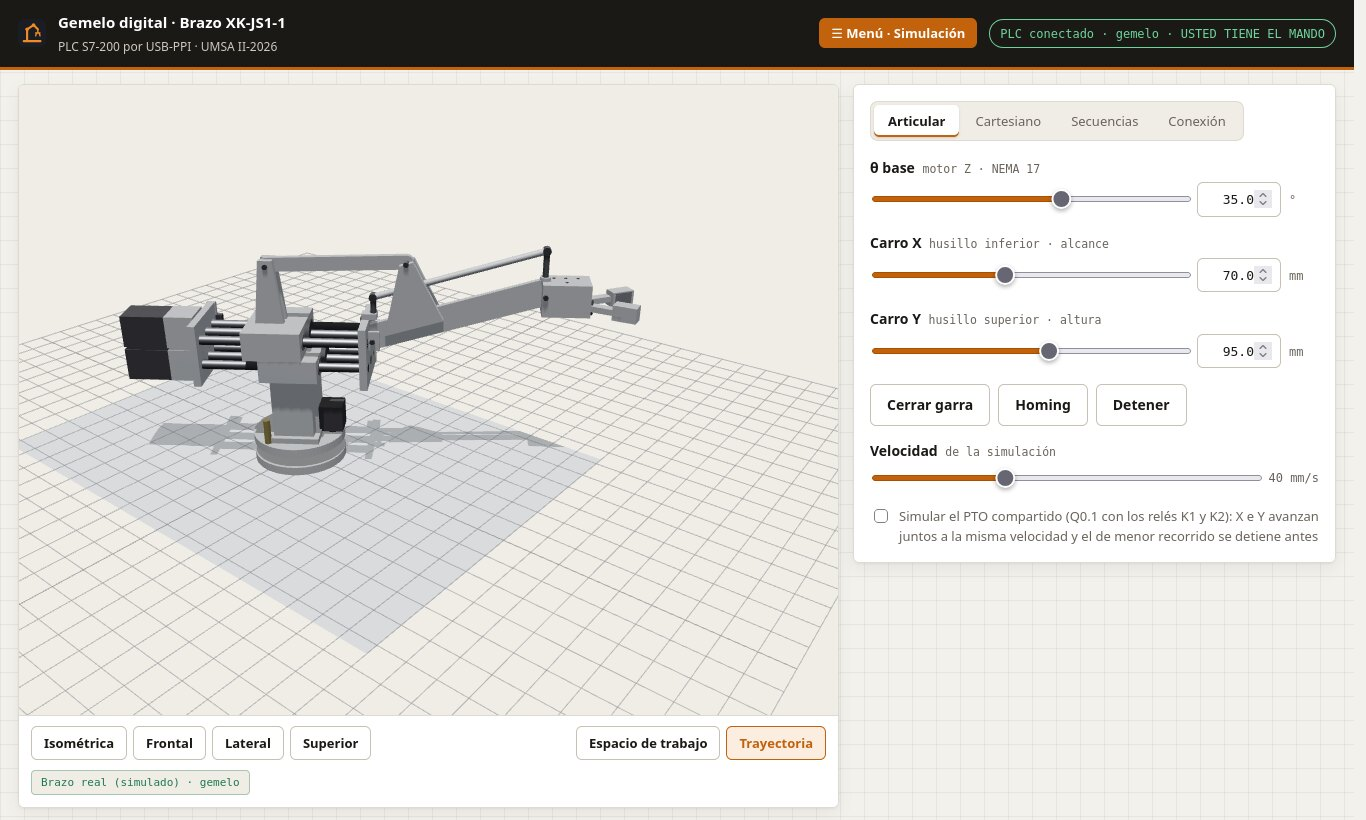
\includegraphics[height=6cm, width=0.62\linewidth, keepaspectratio]{local_articular.jpg}\hfill
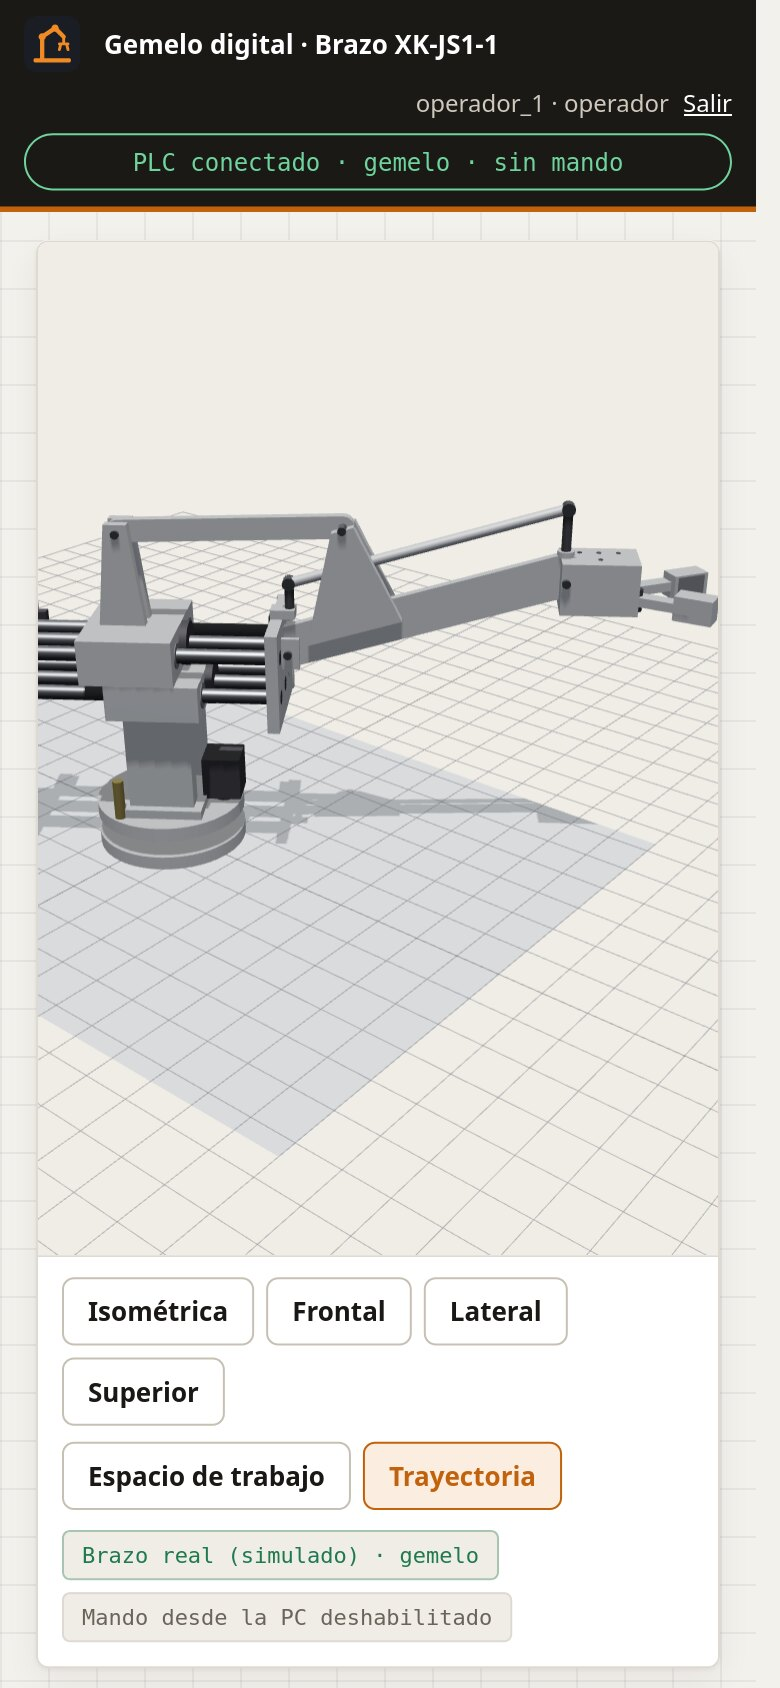
\includegraphics[height=6cm, width=0.34\linewidth, keepaspectratio]{remoto_operador.jpg}
\caption{Interfaz local (izquierda) y vista remota del operador (derecha) de la aplicación.}
\end{figure}

\section{Entregables (Definition of Done)}
\begin{dod}
Plano P\&ID v2.0 (ISA-5.1, cajetín formal) & \cumple & \codigo{documentacion/planos\_isa/pid/brazo\_pid\_v2.dwg} / \codigo{.pdf}\\
Plano eléctrico de potencia y mando (IEC) con bornes al PLC & \cumple & \codigo{documentacion/planos\_isa/electrico/brazo\_electrico\_v2.dwg} / \codigo{.pdf}; quedan puntos SUPUESTO por verificar\\
Prototipo de mockups con paleta y organigrama & \cumple & \codigo{database/mockups/lab2\_mockups\_y\_organigrama.pdf}; falta el enlace al prototipo interactivo\\
Cuadro descriptivo de campos & \cumple & sección 5.2 y documento de base de datos\\
Archivos nativos como anexo & \cumple & DWG, DXF y script generador en \codigo{documentacion/planos\_isa/}\\
\end{dod}

\section{Conclusiones}
\begin{enumerate}
\item El plano histórico tenía seis discrepancias con la planta real (laboratorio 1); las más graves eran las salidas de dirección dibujadas sin conexión y el desfase de las entradas de los finales de carrera. La versión 2.0 las corrige, junto con el tren de pulsos compartido y la numeración de lazos ISA (siete correcciones en total), y las documenta en su tabla de revisión.
\item El P\&ID deja claro que el brazo es un sistema en lazo abierto con supervisión discreta: no hay transmisores continuos de posición. Esa es la limitación principal para los laboratorios de control de la fase 3.
\item Los tags ISA definidos aquí (lazos 100 a 104) son los mismos que usa la base de datos, lo que cumple el requisito de lenguaje común entre control y cómputo.
\item Antes de declarar definitivo el plano eléctrico, hay que verificar los cuatro puntos SUPUESTO en el tablero.
\end{enumerate}

\end{document}
